\documentclass[11pt]{article}
\usepackage [french]{babel}
\usepackage [T1]{fontenc}

\usepackage[linesnumbered, ruled, french, onelanguage]{algorithm2e}
\usepackage{adjustbox}%Permet de centrer les figures dans la largeur de la page même si les figures sont plus larges que \textwidth
\usepackage{amssymb}
\usepackage{amsmath}
\usepackage{adjustbox} % pour avoir adjustbox
\usepackage[toc,page,title,titletoc,header]{appendix}
\usepackage{expl3}%Pour la control sequence /ExlpSyntaxOn demandée par l'utilisation de subfiles apparemment...
\usepackage{gensymb}%pour pouvoir écrire le signe °
%\usepackage{geometry}%Pour changer la largeur des marges du document notamment
\usepackage[paper=a4paper,margin=1in]{geometry}% http://ctan.org/pkg/geometry
\usepackage{graphicx}
\usepackage{hyperref}%pour les liens dans la bibliographie
\usepackage{listings}
\usepackage{placeins}%pour utiliser FloatBarrier afin que les figure respectent bien leur position dans le code
\usepackage{slashbox}%Case séparée en deux tout en haut à gauche des tableaux à double entrées
\usepackage{stmaryrd}%pour les crochets à double barres d'intervalles de nombre entiers
\usepackage{tikz}
\usepackage{xcolor}%/definecolor et /color
\usepackage{subfiles}
\usepackage[useregional]{datetime2}

\usepackage{etoolbox}%pour /AtBeginEnvironment
\AtBeginEnvironment{appendices}{\renewcommand{\thesection}{\Alph {section}}}%Pour recommencer à compter les sections à 0 en rentrant dans l'annexe et pour compter avec des lettres et non des chiffres
\renewcommand{\appendixpagename}{\centering Annexes}%Pour centrer le titre de la partie annexe
\renewcommand{\appendixtocname}{Table des annexes} % Pour faire apparaître les annexes dans la table of contents
\setlength{\parskip}{2mm}%Pour mettre de l'espacement entre les paragraphes

%TODO
% Images qui montrent les différences de résultats pour les différentes tailles de patch size : pour la brique, le pain et le panier

\author{Tom CLABAULT - p2205453\\}
\title{
\noindent\rule{\textwidth}{1pt}
\textit{\textbf{TP Surfaces Implicites}}\\
\noindent\rule{\textwidth}{1pt}
%\vskip 1cm
}
%\date{20 septembre 2023\\}
\geometry{hmargin=1cm, vmargin=0cm}

\begin{document}

\maketitle
%\newgeometry{top=1in,bottom=1in,right=0.5in,left=1.5in}

\section{Surfaces implicites}
        	\begin{figure}[h!]
	\adjustbox{center}{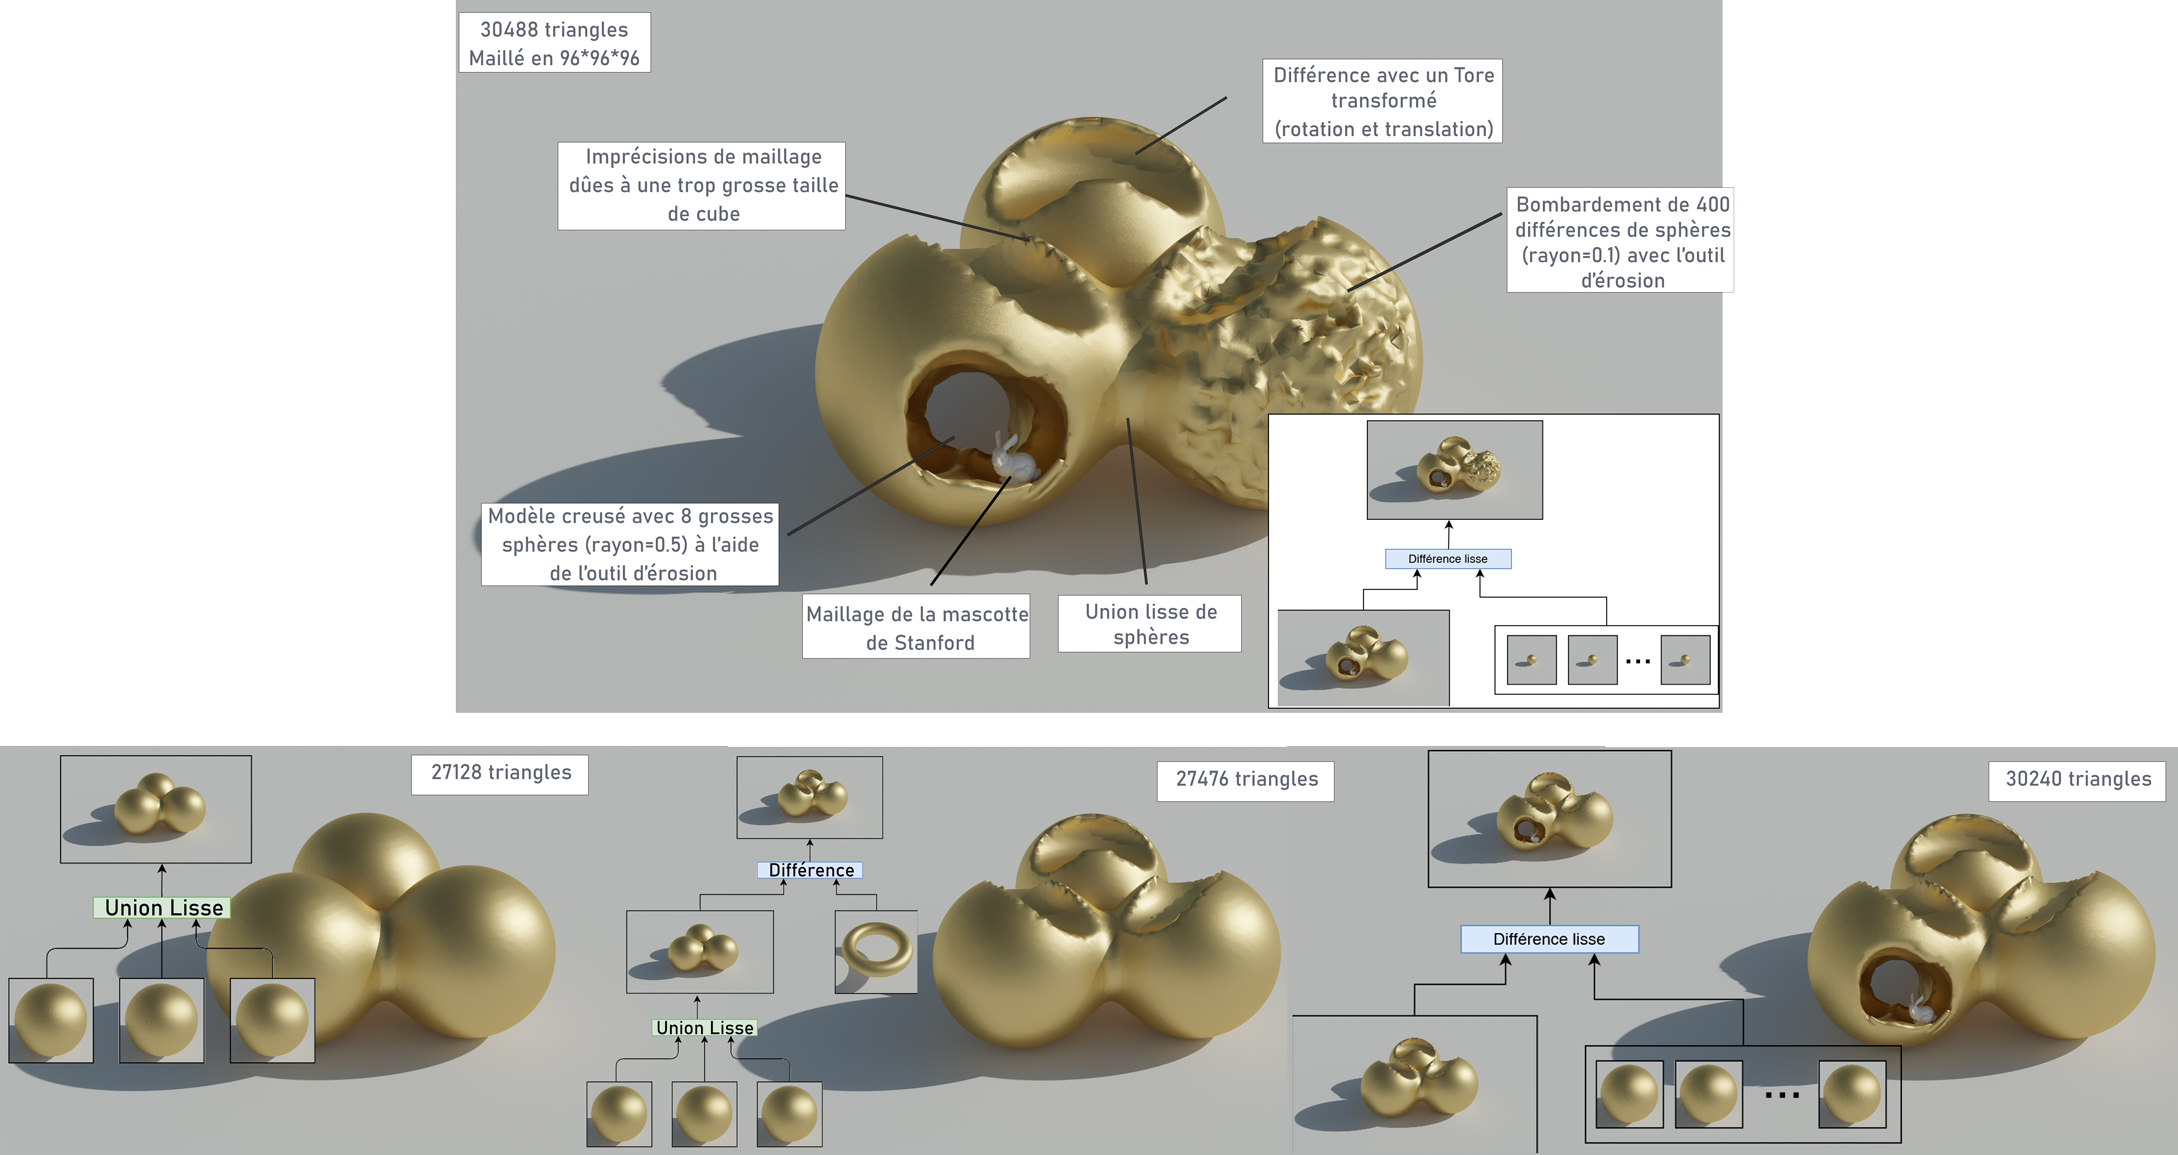
\includegraphics[width=1.2\textwidth]{Captures/DisplayFinal.jpg}}

	\caption{Rendu Blender d'une surface implicite modélisée et maillée avec TinyMesh}
	\label{ref}
\end{figure}
\FloatBarrier

Les opérateurs binaires de modélisation ont été implémentés au moyen de 7 classes, d'héritage de fonctions virtuelles en C++.

La \figurename 1 montre les intéractions possibles avec différents opérateurs binaires de modélisation. Le temps nécessaire ou maillage (ou au rendu par ray-marching) du modèle
dépend directement de la complexité de l'arbre de construction. Pour cet exemple, le plus gros consommateur de temps de calcul est l'outil d'érosion qui peut rajouter jusqu'à
100 différences de sphères à la SDF à chaque clic. Chaque appel à la fonction \textit{Value()} de la SDF doit alors prendre en compte toutes ces nouvelles sphères.

\begin{figure}[h!]
	\adjustbox{center}{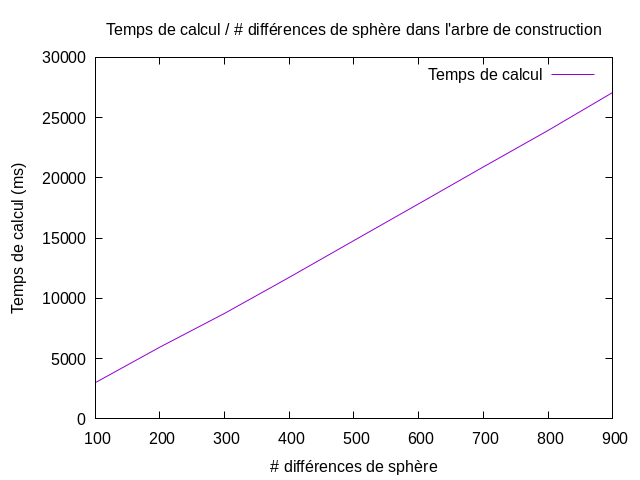
\includegraphics[width=0.8\textwidth]{Benchmark/remesh.png}}

	\caption{Temps d'exécution de l'algorithme de maillage de la surface implicite en fonction de la complexité de la SDF (nombre de différences de sphère utilisé dans la SDF)}
\end{figure}
\FloatBarrier

\subsection {Outil d'érosion}

L'outil d'érosion a été implémenté grâce à un algorithme de ray marching. On lance des rayons aléatoirement autour de la position où l'utilisateur a cliqué
et on rajoute des différences de sphère à la SDF aux points d'intersection. 

L'algorithme de ray marching faisant appel à la fonction \textit{Value()} de la SDF, il est de moins
en moins efficace (linéairement) au fur et à mesure que la SDF se complexifie. Un lancer de rayons classique + BVH sur le maillage de la surface implicite se révèle être 3 
ordres de grandeur plus rapide mais cela nécessite cependant d'avoir maillé la surface implicite au préalable.


\end{document}
